El \textit{algoritmo de Floyd} calcula todos los caminos de coste mínimo \textbf{entre cada par de vértices} del grafo \(G\).
\begin{minted}[breaklines]{C++}
template <typename tCoste> 
matriz<tCoste>
  Floyd(const GrafoP<tCoste>& G, matriz<typename GrafoP<tCoste>::vertice>& P);
\end{minted}

Como salida tenemos:
\begin{itemize}
  \item \textbf{Matriz de costes mínimos} de tamaño \(n*n\), con \(n\) = \texttt{G.numVert()}.
  \item \textbf{Matriz de vértices} (\(P\)) de tamaño \(n*n\), tal que, \texttt{P[i][j]} es un vértice intermedio, por el que pasa el camino de coste mínimo \(i, j\).
\end{itemize}

\begin{figure}[h]
  \begin{center}
    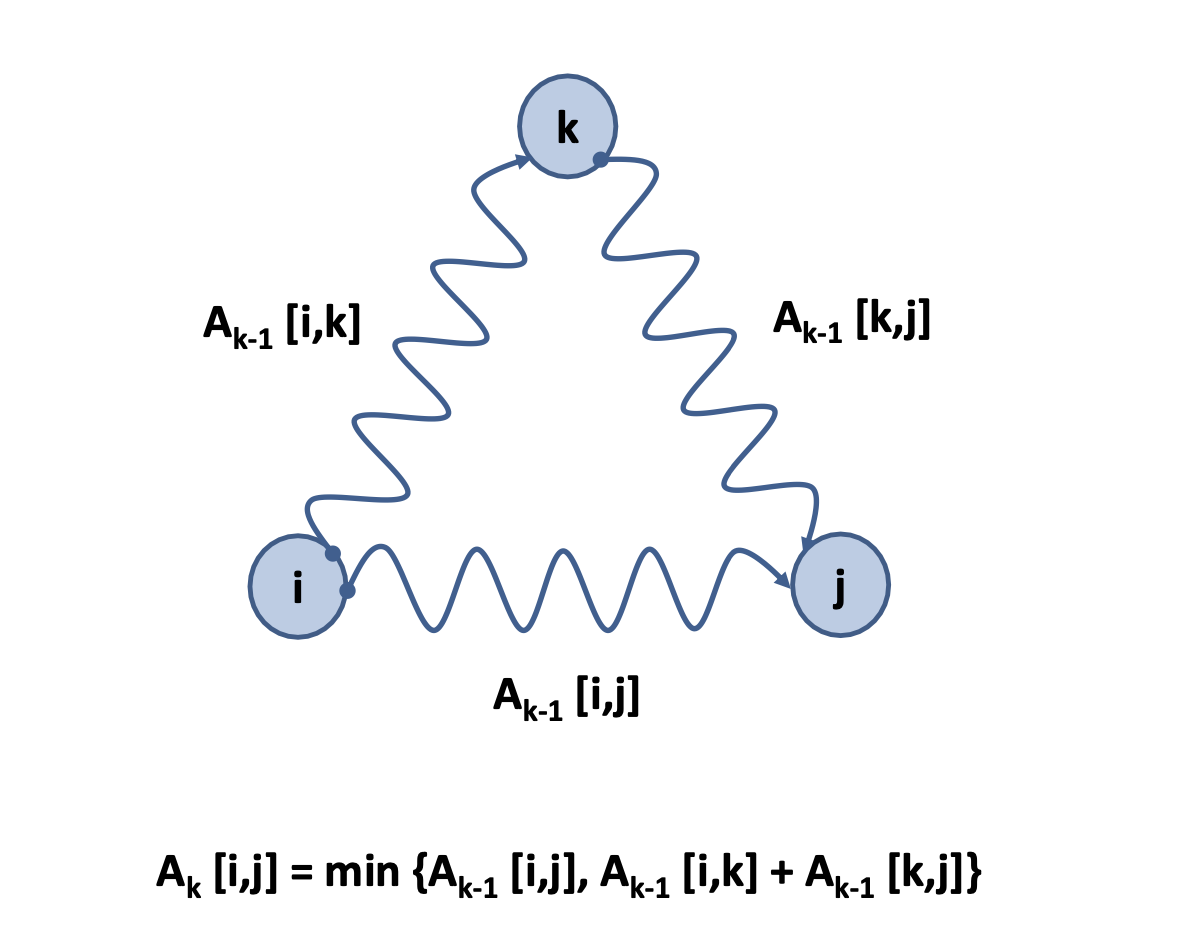
\includegraphics[width=.5\textwidth]{assets/flo1.png}
  \end{center}
El subíndice \(A_{k-1}\) significa la iteración en la que estamos. Siempre nos quedamos con el valor mínimo.
\end{figure}

En \textit{Dijkstra} asumimos que el coste mínimo de ir del origen así mismo es 0. En \textit{Floyd} el equivalente a lo que hacemos en Dijkstra será colocar 0 (n veces), esto se traduce en poner todo a 0 la \textbf{diagonal principal de la matriz de costes mínimos}.

\subsection{Código del algoritmo de Floyd}
\subsubsection{Algoritmo de Floyd}
\begin{minted}[breaklines]{C++}
template <typename tCoste> 
matriz<tCoste> Floyd(const GrafoP<tCoste>& G, matriz<typename GrafoP<tCoste>::vertice>& P){
  typedef typedef GrafoP<tCoste>::vertice vertice;
  const size_t n = G.numVert();
  matriz<tCoste> A(n); //matriz de costes mínimos
//Iniciamos A y P con caminos directos entre cada par de vértices
  P = matriz<vertice>(n); //creamos una matriz de vertices
  for(vertice i = 0; i<= n-1 ; i++){
    A[i] = G[i]; //copiamos los costes del grafo
    A[i][i] = 0; //diagonal principal a 0.
    P[i] = vector<vertice>(n,i); //caminos directos
  }
//Calcular costes minimos y caminos correspondientes
//entre cualquier par de vértices i, j
  for(vertice k = 0; k <= n-1; k++)
    for(vertice i = 0; i <= n-1; i++)
      for(vertice j = 0; j<=n-1; j++){
        tCoste ikj = suma(A[i][k], A[k][j]);
        if(ikj < A[i][j]){ //optimización de los costes minimos
          A[i][j] = ikj;
          P[i][j] = k;
        }
      }
  return A; //devolvemos la matriz de costes
}
\end{minted}

Cosas a tener en cuenta del código:
\begin{itemize}
  \item Con \texttt{A[i] = G[i]} \(\rightarrow\) copiamos los costes del Grafo en la matriz entrante.
  \item Con \texttt{A[i][i] = 0} \(\rightarrow\) hacemos que el coste mínimo de ir a donde estamos nosotros mismos sea 0, es decir la \textbf{diagonal principal} de la matriz (como hemos comentado anteriormente).
  \item Con \texttt{P[i] = vector<vertice>(n,i)} \(\rightarrow\) asignamos a P[i] un vector de vértices por los que pasa.
  \item La variable \texttt{ikj} \(\rightarrow\) es la suma de los costes mínmos de ir desde un vértice \(i\) a otro \(j\) pasando por \(k\), es decir, \texttt{ikj = suma(A[i][k], A[k][j])}. 
  \item Si la suma de estos costes es menor que el coste del grafo `\texttt{A[i][j]}', es decir (\texttt{ikj < A[i][j]}), podemos optimizar el coste de ir de \(i \rightarrow j\).
\end{itemize}

\subsubsection{Método Camino}
Este método devuelve una lista de vértices entre dos vértices cualesquiera:

\begin{minted}[breaklines]{C++}
template <typename tCoste> typename GrafoP<tCoste>::tCamino caminoAux(typename GrafoP<tCoste>::vertice v, typename GrafoP<tCoste>::vertice w, const matriz<typename GrafoP<tCoste>::vertice>& P){
// Devuelve el camino de coste mínimo entre v y w, exluidos estos,
// a partir de una matriz P obtenida mediante la función Floyd().
  typename GrafoP<tCoste>::tCamino C1, C2;
  typename GrafoP<tCoste>::vertice u;
  u = P[v][w];
  if(u != w){
    C1 = caminoAux<tCoste>(v,u,P);
    C1.insertar(u,C1.fin());
    C2 = caminoAux<tCamino(u,w,P);
    C1 += C2; //lista<vertice>::operator *=(), concatena C1 y C2.
  }
  return C1; /7/devolvemos la lista
}

template <typename tCoste> typename GrafoP<tCoste>::tCamino camino(typename GrafoP<tCoste>::vertice v, typename GrafoP<tCoste>::vertice w, const matriz<typename GrafoP<tCoste>::vertice>& P){
// Devuelve el camino de coste mínimo desde v hasta w a partir
// de una matriz P obtenida mediante la función Floyd().
  typename GrafoP<tCoste>::tCamino C;
  C = caminoAux<tCoste>(v,w,P);
  C.insertar(v,C.primera());
  C.insertar(w,C.fin());
  return C;
}
\end{minted}

Cosas a tener en cuenta del código del método \textit{caminoAux}:
\begin{itemize}
  \item El vértice \texttt{u} es el último vértice que se ha utilizado para optimizar el camino entre los vértices \(v\) y \(w\).
  \item Mediante \texttt{C1 = caminoAux<tCoste>(v,u,P)} \(\rightarrow\) calculamos el camino desde el vértice \(v\) hasta el vértice \(u\).
  \item Mediante \texttt{C2 = caminoAux<tCamino(u,w,P)} \(\rightarrow\) calculamos el camino desde el vértice \(u\) hasta el vértice \(w\).
  \item Con \texttt{C1 += C2} \(\rightarrow\) concatenamos los caminos en la lista de vértices.
 \end{itemize}
En este método vemos que solamente insertamos el último vértice por el que se ha pasado en el camino \(v \rightarrow w\), es decir, \(u\).
